% from 
% https://tex.stackexchange.com/a/232723/235813

% https://mirror.mwt.me/ctan/macros/latex/contrib/bookcover/bookcover.pdf
% https://mirror.math.princeton.edu/pub/CTAN/macros/latex/contrib/bookcover/bookcover.pdf

\documentclass[marklength=0mm,
    coverwidth=148.5mm,
    coverheight=210mm,
    bleedwidth=0mm,
    spinewidth=10mm]{bookcover}

% https://tex.stackexchange.com/a/31309/235813
\hyphenpenalty=10000

\usepackage{graphicx}
%\usepackage{setspace} % doublespace

\begin{document}

%back cover
\setbookcover{bgcolor}{back}{%
color=blue!20,
}


\setbookcover{fgfirst}{back}{%
\centering
%\begin{minipage}[c]{.7\textwidth}
%{
\vspace*{2cm}
{\Large Why doesn't everything just work better?!}
\vspace*{2cm}

\parbox{11cm}{If most people want to do the right thing, why do the organizations society relies on perpetually operate in suboptimal modes? Good people collaborating on complex challenges consistently yield less-than-ideal outcomes. 

\ \\
More immediate to you, your choices are constrained by the decisions of people you may not directly interact with. 
As the population increases and we live closer to each other, shared resources become scarcer, the need for coordination becomes more important.

\ \\
When you're faced with bureaucracy that ranges from mundane and trivial to the Kafkaesque-level, this guidebook empowers you to be more effective. }
\vfill
\parbox{9cm}{Ben Payne brings his decades of experience as a professional bureaucrat to illuminate the confusing aspects of everyday life. Ben draws on his military background, participation in small companies, and time in the Federal government.}
\vfill

% https://www.creativindiecovers.com/free-online-isbn-barcode-generator/
\parbox{12cm}{\begin{flushright}
    
\includegraphics{isbn_10usd.pdf}
\end{flushright}}


%\blindtext
%\end{minipage}
}

%front cover
\setbookcover{bgcolor}{front}{%
color=olive!30, % https://en.wikibooks.org/wiki/LaTeX/Colors
}

\setbookcover{fgsecond}{front}{%
\vspace{3cm}
\centering
%\scalebox{3}{\drawduck}
\vfill
}

\setbookcover{fgfirst}{front}{%
\centering
%\begin{minipage}[c]{.4\textwidth}
\vfill 
% each \vfill will expand vertically the same amount until the entire page is filled.
% https://tex.stackexchange.com/a/13920/235813
\begin{center}
%\begin{doublespace}
{\Huge Process Empathy:}\\
\vspace*{.5cm}
{\Huge The Field Guide for}\\
\vspace*{.5cm}
{\Huge Effective Bureaucrats}\\
\vfill
% https://tex.stackexchange.com/a/57420/235813
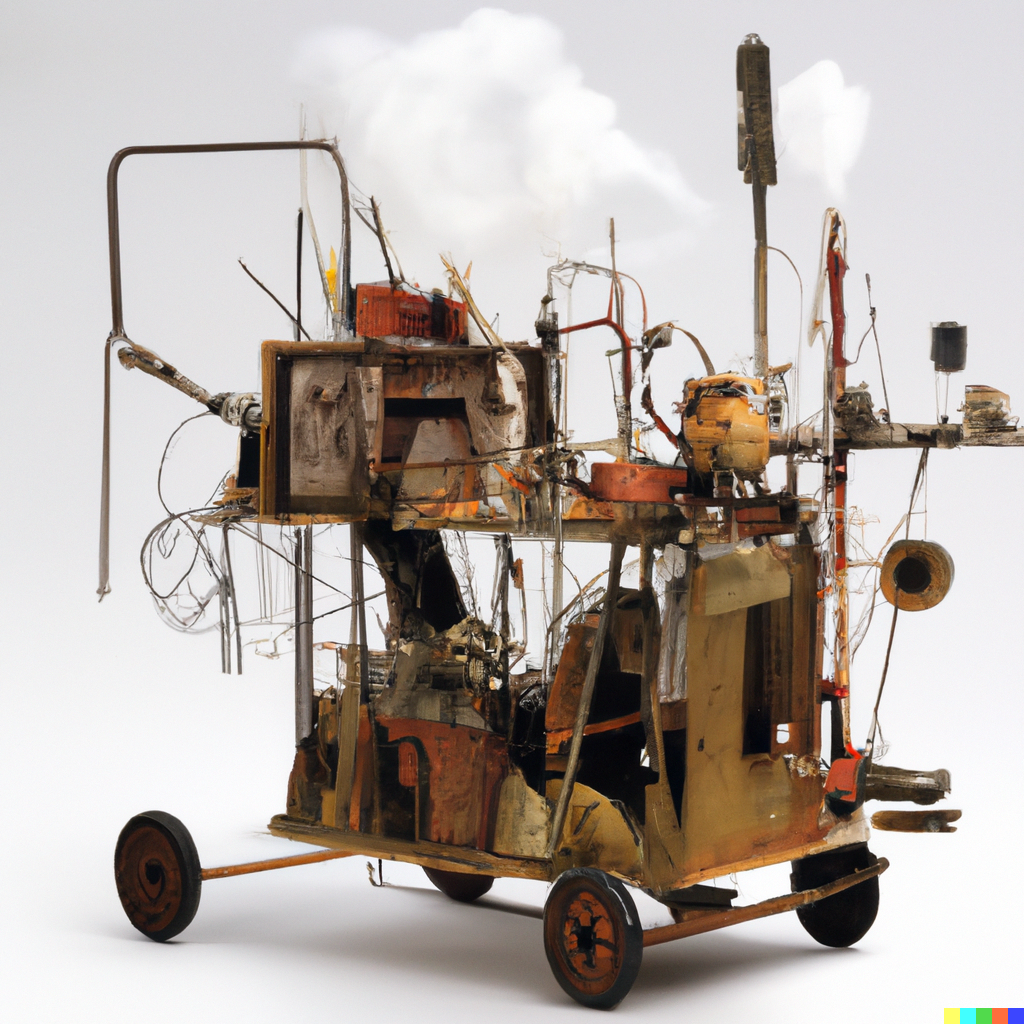
\includegraphics[width=10cm,trim={2cm 0.8cm 0 0},clip]{DALLE_2023-01-14_21-10-38_complicated_mechanical_device_made_of_electronics_and_brass}
\vfill
{\Huge Ben Payne}
\vfill
\end{center}
%\end{minipage}
}

%spine
\setbookcover{bgcolor}{spine}{%
color=yellow!50,
}

\setbookcover{fgfirst}{spine}{
\vfill
\centering
\rotatebox[origin=c]{-90}{
\begin{tabular}{c}
{\Large Process Empathy: The Field Guide for Effective Bureaucrats}
\end{tabular}
\hspace{2cm}
{\Large Ben Payne}
}
\vfill}

\makebookcover
\end{document}